% !TEX TS-program = pdflatex
% !TEX encoding = UTF-8 Unicode

% This is a simple template for a LaTeX document using the "article" class.
% See "book", "report", "letter" for other types of document.

\documentclass[11pt]{article} % use larger type; default would be 10pt

\usepackage[utf8]{inputenc} % set input encoding (not needed with XeLaTeX)
\usepackage[document]{ragged2e}

%%% Examples of Article customizations
% These packages are optional, depending whether you want the features they provide.
% See the LaTeX Companion or other references for full information.

%%% PAGE DIMENSIONS
\usepackage{geometry} % to change the page dimensions
\geometry{a4paper} % or letterpaper (US) or a5paper or....
% \geometry{margin=2in} % for example, change the margins to 2 inches all round
% \geometry{landscape} % set up the page for landscape
%   read geometry.pdf for detailed page layout information

\usepackage[table,xcdraw]{xcolor}

\usepackage{graphicx} % support the \includegraphics command and options
\usepackage{enumerate}

% \usepackage[parfill]{parskip} % Activate to begin paragraphs with an empty line rather than an indent

%%% PACKAGES
\usepackage{booktabs} % for much better looking tables
\usepackage{array} % for better arrays (eg matrices) in maths
\usepackage{paralist} % very flexible & customisable lists (eg. enumerate/itemize, etc.)
\usepackage{verbatim} % adds environment for commenting out blocks of text & for better verbatim
\usepackage{subfig} % make it possible to include more than one captioned figure/table in a single float
% These packages are all incorporated in the memoir class to one degree or another...

%%% HEADERS & FOOTERS
\usepackage{fancyhdr} % This should be set AFTER setting up the page geometry
\pagestyle{fancy} % options: empty , plain , fancy
\renewcommand{\headrulewidth}{0pt} % customise the layout...
\lhead{}\chead{}\rhead{}
\lfoot{}\cfoot{\thepage}\rfoot{}

\usepackage{xcolor}

%%% SECTION TITLE APPEARANCE
\usepackage{sectsty}
\allsectionsfont{\sffamily\mdseries\upshape} % (See the fntguide.pdf for font help)
% (This matches ConTeXt defaults)

%%% ToC (table of contents) APPEARANCE
\usepackage[nottoc,notlof,notlot]{tocbibind} % Put the bibliography in the ToC
\usepackage[titles,subfigure]{tocloft} % Alter the style of the Table of Contents
\renewcommand{\cftsecfont}{\rmfamily\mdseries\upshape}
\renewcommand{\cftsecpagefont}{\rmfamily\mdseries\upshape} % No bold!
\usepackage{amsmath,amssymb}

%%% END Article customizations

%%% The "real" document content comes below...

\title{Métodos Determinísticos de Investigação Operacional \\ \large Trabalho Prático}
\author{Diogo Sobral, a82523 \\ Henrique Pereira, a80261 \\ Pedro Moreira, a82364 \\ Pedro Ferreira, a81135}
\date{2018/2019}

\begin{document}
\maketitle

\begin{figure*}[!b]
    \centering
    
\includegraphics[width=1in]{um_eeng.jpg}
\end{figure*}

\newpage

\section*{Questão 1}
\subsection*{a)}
\textbf{Parâmetros:}  \\
\begin{center}
n - número de nodos existentes \\
c\textsubscript{ij} - tempo de propagação no arco ij\\
i=1,...,n e j=1,...n \\
\end{center}
\textbf{Variáveis de Decisão:} \\
\begin{center}
x\textsubscript{ij} - número de caminhos a que o arco que une os nodos i e j pertence\\
i=1,...,n e j=1,...n \\
\end{center}
\textbf{Função Objetivo:} \\
$$min \ Z = \sum_{i=1}^{n} \sum_{j=1}^{n} c_i_jx_i_j$$
\textbf{Sujeito a:}
\begin{enumerate}[(i)]
\item $$x_i_i = 0, \forall i \in 1,...,n$$
\item $$\sum_{j=2}^{n} (x_1_j - x_j_1) = n-1$$
\item $$\sum_{j=1}^{n} (x_i_j - x_j_i) = -1, \forall i \in 2,...,n $$
\item $$x_i_j \geq 0, \forall i \in 1,...,n , \forall j \in 1,...,n$$
\end{enumerate}\\


Neste modelo, a função objetivo procura que o tempo de chegada do fogo a cada um dos nodos seja o mínimo possível pois serão considerados os arcos de menor custo. Uma vez que a variável de decisão representa o número de caminhos a que o arco ij pertence, o conjunto dos arcos com origem no nodo de ignição, ou seja, no nodo 1,  têm de necessariamente pertencer a todos os caminhos existentes. A restrição (ii) expressa esta condição. Nos restantes nodos, o conjunto dos arcos com origem num determinado nodo i pertencem a menos um caminho que o conjunto dos nodos que chegam a i. Esta situação é definida pela restrição (iii). A equação (i) representa o facto de não existirem arcos cuja origem e destino sejam o mesmo nodo. Por fim, a restrição (iv) estabelece a não negatividade das variáveis.\\
\textcolor{red}{Falta exemplificar com a instância}

\subsection*{b)}

\textbf{Parâmetros:}  \\
\begin{center}
n - número de nodos existentes \\
c\textsubscript{ij} - tempo de propagação no arco ij\\
i=1,...,n e j=1,...n \\
\end{center}
\textbf{Variáveis de Decisão:} \\
\begin{center}
t\textsubscript{i} - tempo decorrido desde a ignição aquando da chegada do fogo ao nodo i\\
i=1,...,n\\
\end{center}
\textbf{Função Objetivo:} \\
$$max \ Z = \sum_{i=1}^{n} t_i$$
\textbf{Sujeito a:}
\begin{enumerate}[(i)]
\item $$t_1 = 0$$
\item $$t_j \leq t_i + t_i_j, \forall i \in 1,...,n , \forall j \in 2,...,n$$
\item $$t_i \geq 0, \forall i \in 1,...,n$$
\end{enumerate}

Enquanto que o modelo primal tinha em consideração o número de caminhos a que um determinado arco pertencia, no modelo duas a variável de decisão representa o momento em que o fogo atinge um determinado nodo. Considerando a ignição no nodo 1, surge a restrição (i). Em conjunto com a função objetivo, a restrição (ii) garante que o tempo de chegada a cada nodo é o mínimo possível, tendo em conta a formulação do problema. Por um lado, queremos maximizar o tempo de chegada a cada nodo (função objetivo), por outro, pela restrição (ii), garante-se que o momento de chegada a um nodo j não é anterior ao menor dos tempos chegada ao conjunto dos nodos adjacentes a j, somado do custo de propagação para este. Por fim, a restrição (iii) estabelece a não negatividade das variáveis.

\textcolor{red}{Falta exemplificar com a instância}

\subsection*{c)}
\textcolor{red}{Obtenha as soluções óptimas primal e dual através da resolução do modelo primal.}

\subsection*{d)}
\textcolor{red}{Obtenha as soluções óptimas primal e dual através da resolução do modelo dual. Confirme que as soluções são as mesmas que as obtidas na alínea anterior, ou, caso não sejam, apresente uma justificação.}

\section*{Questão 2}
\subsection*{a)}
\textbf{Parâmetros:}  \\
\begin{center}
n - número de nodos existentes \\
Q\textsubscript{k} - Nodos adjacentes a k \\
k=1,...,n \\
c\textsubscript{ij} - tempo de propagação no arco ij\\
i=1,...,n e j=1,...n \\
b - número de recursos disponíveis \\
$\Delta$ - constante de retardação \\
ignição - célula de ignição do fogo \\
objetivo - célula a que se pretende atrasar a chegada do fogo
\end{center}

\textbf{Variáveis de Decisão:} \\
\begin{center}
x\textsubscript{i} = \begin{cases} 1, & \mbox{se é aplicado um recurso de proteção na célula i}  \\  0, & \mbox{caso contrário} \end{cases} \\
i=1,...,n \\
t\textsubscript{i} - tempo decorrido desde a ignição aquando da chegada do fogo ao nodo i \\
i=1,...,n \\
\end{center}
\textbf{Função Objetivo:} \\
$$max \ Z = t\textsubscript{$objetivo$}$$ \\

\textbf{Sujeito a:}
\begin{enumerate}[(i)]
\item $$t\textsubscript{ignição} = 0$$
\item $$t_j \leq t_i + c_i_j + \Delta * x_i, \forall i \in Q\textsubscript{j} , \forall j \in 1,...,n$$
\item $$\sum_{i=1}^{n} x_i \leq b$$
\item $$t_i \geq 0, \forall i \in 1,...,n$$
\end{enumerate}
O objetivo do problema é escolher onde aplicar recursos de proteção, que atrasam a propagação do fogo, de forma a retardar o máximo possível o momento de chegada do fogo a um determinado nodo (nodo objetivo). Para alcançar esse fim, consideramos como variável de decisão o tempo de chegada do fogo a cada nodo. Logo, a função objetivo procura maximizar o tempo de chegada ao nodo objetivo. Uma vez que a célula de ignição é um parâmetro do problema e não um valor fixo, temos de associar matematicamente o início do fogo ao nodo de ignição. A restrição (i) garante essa associação. A restrição (ii), em conjunto com a função objetivo, assegura a correta aplicação dos recursos de proteção, em função da célula que queremos proteger. Uma vez que o tempo de chegada do fogo a um certo nodo é definido por recorrência, isto é, o momento de chegada a um nodo j define-se à custa do tempo de chegada a outro nodo e assim sucessivamente até alcançarmos o nodo de ignição, único que se define a si mesmo, o modelo optará por colocar proteções em células que façam parte do caminho percorrido pelo fogo até ao nodo que queremos proteger, maximizando o tempo de chegada a este. A restrição(iii) limita o número de recursos aplicados e a restrição (iv) define a não negatividade das variáveis.
A função objetivo traduz a finalidade pretendida.
\subsection*{b)}
\begin{table}[h]
\centering
\begin{tabular}{cccccccc}
i\textbackslash{}j     & 1                                               & 2                                               & 3                                               & 4                                               & 5                                               & 6                                               & 7                                               \\ \cline{2-8}
\multicolumn{1}{c|}{1} & \multicolumn{1}{c|}{\cellcolor[HTML]{FFFFFF}0}  & \multicolumn{1}{c|}{\cellcolor[HTML]{FFFFFF}13} & \multicolumn{1}{c|}{\cellcolor[HTML]{FFFFFF}25} & \multicolumn{1}{c|}{\cellcolor[HTML]{F8FF00}36} & \multicolumn{1}{c|}{\cellcolor[HTML]{F8FF00}39} & \multicolumn{1}{c|}{\cellcolor[HTML]{F8FF00}42} & \multicolumn{1}{c|}{\cellcolor[HTML]{F8FF00}43} \\ \cline{2-8}
\multicolumn{1}{c|}{2} & \multicolumn{1}{c|}{\cellcolor[HTML]{FFFFFF}15} & \multicolumn{1}{c|}{\cellcolor[HTML]{FFFFFF}27} & \multicolumn{1}{c|}{\cellcolor[HTML]{F8FF00}39} & \multicolumn{1}{c|}{\cellcolor[HTML]{F8FF00}41} & \multicolumn{1}{c|}{\cellcolor[HTML]{F8FF00}45} & \multicolumn{1}{c|}{\cellcolor[HTML]{F8FF00}48} & \multicolumn{1}{c|}{\cellcolor[HTML]{F8FF00}50} \\ \cline{2-8}
\multicolumn{1}{c|}{3} & \multicolumn{1}{c|}{\cellcolor[HTML]{FFFFFF}31} & \multicolumn{1}{c|}{\cellcolor[HTML]{F8FF00}41} & \multicolumn{1}{c|}{\cellcolor[HTML]{F8FF00}44} & \multicolumn{1}{c|}{\cellcolor[HTML]{F8FF00}49} & \multicolumn{1}{c|}{\cellcolor[HTML]{F8FF00}51} & \multicolumn{1}{c|}{\cellcolor[HTML]{F8FF00}55} & \multicolumn{1}{c|}{\cellcolor[HTML]{F8FF00}57} \\ \cline{2-8}
\multicolumn{1}{c|}{4} & \multicolumn{1}{c|}{\cellcolor[HTML]{F8FF00}45} & \multicolumn{1}{c|}{\cellcolor[HTML]{F8FF00}48} & \multicolumn{1}{c|}{\cellcolor[HTML]{F8FF00}52} & \multicolumn{1}{c|}{\cellcolor[HTML]{F8FF00}55} & \multicolumn{1}{c|}{\cellcolor[HTML]{F8FF00}58} & \multicolumn{1}{c|}{\cellcolor[HTML]{F8FF00}61} & \multicolumn{1}{c|}{\cellcolor[HTML]{F8FF00}65} \\ \cline{2-8}
\multicolumn{1}{c|}{5} & \multicolumn{1}{c|}{\cellcolor[HTML]{F8FF00}52} & \multicolumn{1}{c|}{\cellcolor[HTML]{F8FF00}54} & \multicolumn{1}{c|}{\cellcolor[HTML]{F8FF00}57} & \multicolumn{1}{c|}{\cellcolor[HTML]{F8FF00}62} & \multicolumn{1}{c|}{\cellcolor[HTML]{F8FF00}65} & \multicolumn{1}{c|}{\cellcolor[HTML]{F8FF00}69} & \multicolumn{1}{c|}{\cellcolor[HTML]{F8FF00}72} \\ \cline{2-8}
\multicolumn{1}{c|}{6} & \multicolumn{1}{c|}{\cellcolor[HTML]{F8FF00}57} & \multicolumn{1}{c|}{\cellcolor[HTML]{F8FF00}60} & \multicolumn{1}{c|}{\cellcolor[HTML]{F8FF00}63} & \multicolumn{1}{c|}{\cellcolor[HTML]{F8FF00}66} & \multicolumn{1}{c|}{\cellcolor[HTML]{F8FF00}71} & \multicolumn{1}{c|}{\cellcolor[HTML]{F8FF00}74} & \multicolumn{1}{c|}{\cellcolor[HTML]{FFFFFF}77} \\ \cline{2-8}
\multicolumn{1}{c|}{7} & \multicolumn{1}{c|}{\cellcolor[HTML]{F8FF00}59} & \multicolumn{1}{c|}{\cellcolor[HTML]{F8FF00}64} & \multicolumn{1}{c|}{\cellcolor[HTML]{F8FF00}69} & \multicolumn{1}{c|}{\cellcolor[HTML]{F8FF00}73} & \multicolumn{1}{c|}{\cellcolor[HTML]{F8FF00}77} & \multicolumn{1}{c|}{\cellcolor[HTML]{FFFFFF}80} & \multicolumn{1}{c|}{\cellcolor[HTML]{32CB00}92} \\ \cline{2-8}
\end{tabular}
\caption{Representação gráfica da redes de nodos com os tempos da solução obtida.}
\end{table}
\begin{itemize}[$\ast$]
	\item As células a branco representam os nodos onde foram gastos os recursos.
    \item As células a amarelo são nodos normais.
    \item A célula a verde é o nodo a ser protegido.
\end{itemize}
\par A tabela 1 mostra os tempos de chegada do fogo a cada célula a partir do nodo 1. A branco estão representados os locais onde foram colocados os recursos, a verde o nodo a proteger e os restantes a amarelo. Durante a construção deste modelo, deparamo-nos diversas vezes com valores em algumas células que eram díficeis de explicar especialmente quando eram usados poucos recursos. Estes valores levantavam alguma confusão uma vez que, o seu valor não era necessariamente o tempo de chegada do fogo ao nodo mas, por vezes, um valor inferior ao mesmo. Após vários testes para verificar a robustez do modelo, chegamos à conclusão que o OPL só tem os tempos de chegada a um nodo corretos para aqueles que concorrem para a solução do problema, isto é, se a solução não passa por percorrer um dado nodo, muitas vezes este fica com um tempo inferior já que, o seu tempo não vai afetar o objetivo.

\subsection*{c)}
\begin{figure*}[h]
    \centering
    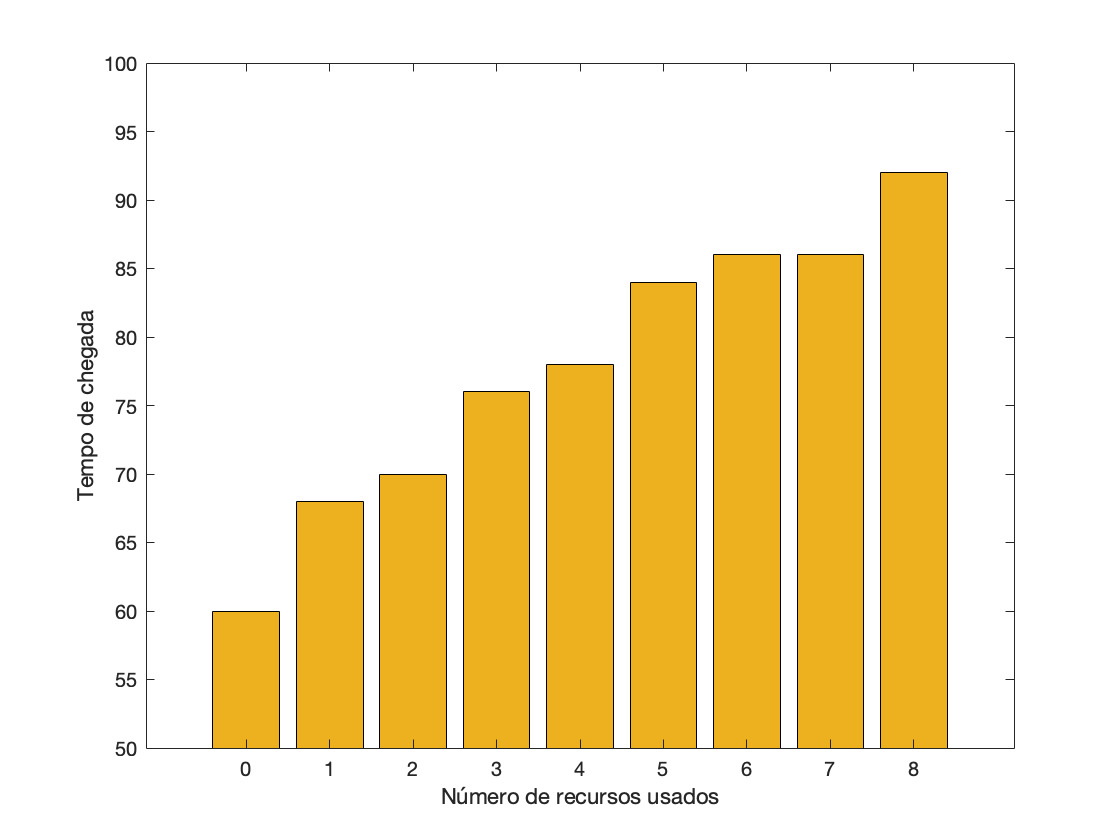
\includegraphics[scale=0.3]{graf2.png}
    \caption{Gráfico Recursos usados - Tempo de chegada}
\end{figure*}

\par Na figura 1 está representado um gráfico que faz uma associação entre o número de recursos utilizados e o respetivo tempo de chegada. Para esta experiência, consideramos o número de recursos disponíveis entre 0 e 8. Com podemos ver acima, inicialmente o tempo de chegada está situado em 60 e este varia até 92. As maiores subidas dão-se quando são utilizados  1,5,8 recursos. \textcolor{red}{Isto tem que meter melhor amanhã acabo}

\section*{Questão 3}

\subsection*{a)}
\textbf{Parâmetros:}  \\
\begin{center}
n - número de nodos existentes \\
c\textsubscript{ij} - tempo de propagação no arco ij\\
i=1,...,n e j=1,...n \\
t\textsubscript{max} - intervalo de tempo considerado\\
b - número de recursos disponíveis \\
$\Delta$ - constante de retardação \\
p\textsubscript{s} - probabilidade de ignição na célula s\\
s=1,...n \\
\end{center}
\textbf{Variáveis de Decisão:} \\

\begin{center}
x\textsubscript{i} = \begin{cases} 1, & \mbox{se é aplicado um recurso de proteção no nodo i}\\ 0, & \mbox{caso contrário}\end{cases} \\
i=1,...,n \\
t\textsubscript{sj} - tempo decorrido aquando da chegada de um fogo, com origem em s, ao nodo i\\
s=1,...,n e i=1,...,n \\
y\textsubscript{si} = \begin{cases} 1, & \mbox{se o fogo com início no nodo} \ s \ \mbox{chega a} \ i \  \mbox{num tempo inferior a t\textsubscript{max}} \\ 0, & \mbox{caso contrário}\end{cases} \\
s=1,...,n e i=1,...,n
\end{center}

\textbf{Função Objetivo:} \\
$$min \ Z = \sum_{s=1}^{n} \sum_{i=1}^{n} p_sy_s_i$$ \\


\textbf{Sujeito a:}
\begin{enumerate}[(i)]
\item $$t\textsubscript{ss} = 0, \forall s \in 1,...,n$$
\item $$t_s_j \leq t_s_i + d_i_j + \Delta x_i, \forall s \in 1,...n, \forall i \in 1,...,n , \forall j \in 1,...,n$$
\item $$y_s_i \geq \frac{ t\textsubscript{max}-t_s_i}{t\textsubscript{max}}, \forall s \in 1,...,n, \forall i \in 1,...,n $$
\item $$\sum_{i=1}^{n} x_i \leq b$$
\end{enumerate}

\subsection*{b)}
\textcolor{red}{Para a instância em anexo, obtenha uma solução através do IBM ILOG CPLEX
Optimization Studio com probabilidade de ignição na célula (i, j) dada por (14 - i -
j)/500 e intervalo de 12 unidades de tempo. Represente a solução de forma adequada
e interprete-a.}

\subsection*{c)}
\textcolor{red}{Represente graficamente o valor esperado da área ardida em função do intervalo
de tempo considerado. Interprete e comente.}

\end{document}
